% 3D Gaussian hot spot -- case_3d_hotspot.py.
% Cube with isothermal walls; a Gaussian blob at the center,
%   T = T0 + A exp(-r^2 / 2 sigma0^2),  sigma0 = 0.08,
% diffuses as the heat-kernel Green's function (spherical-symmetry check):
%   sigma^2(t) = sigma0^2 + 2 alpha t,  peak ~ (sigma0/sigma)^3.
% Run until sigma doubles.
%
% Compile:  pdflatex setup_3d_hotspot.tex
\documentclass[border=6pt]{standalone}
\usepackage{amsmath}
\usepackage{tikz}
\usetikzlibrary{arrows.meta, calc}

\definecolor{coldc}{RGB}{46,86,149}
\definecolor{hotc}{RGB}{171,57,52}
\definecolor{inkc}{RGB}{30,30,30}

\begin{document}
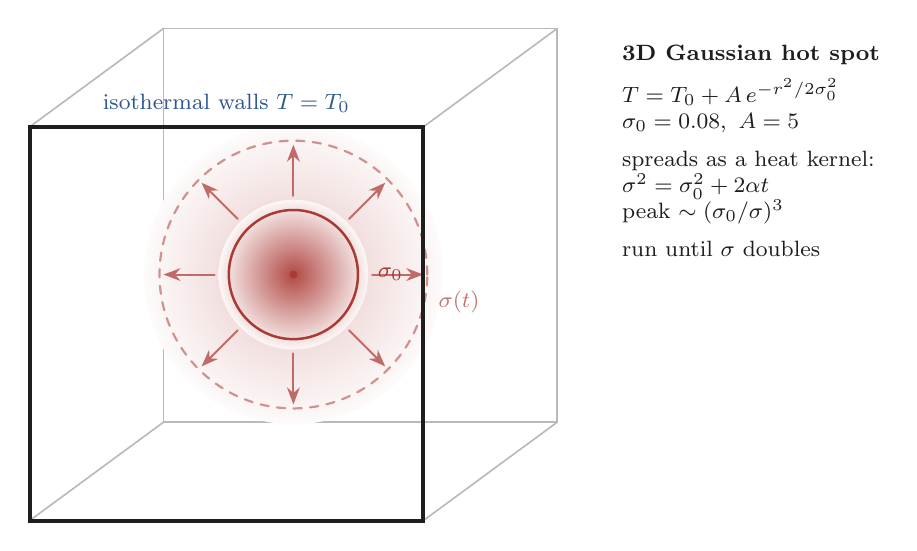
\begin{tikzpicture}[>=Stealth, font=\footnotesize, line cap=round]
  \def\S{5}
  \def\dx{1.7}
  \def\dy{1.25}
  \coordinate (C) at (\S/2+\dx/2,\S/2+\dy/2);  % blob at the cube's visual center (front center + half depth)

  % cube back face + connecting edges
  \draw[gray!55, line width=0.6pt]
    (\dx,\dy) -- (\S+\dx,\dy) -- (\S+\dx,\S+\dy) -- (\dx,\S+\dy) -- cycle;
  \draw[gray!55, line width=0.6pt] (0,0)--(\dx,\dy);
  \draw[gray!55, line width=0.6pt] (\S,0)--(\S+\dx,\dy);
  \draw[gray!55, line width=0.6pt] (\S,\S)--(\S+\dx,\S+\dy);
  \draw[gray!55, line width=0.6pt] (0,\S)--(\dx,\S+\dy);

  % spread state (later, sigma doubled): broad faint blob + dashed extent
  \shade[inner color=hotc!30, outer color=hotc!2] (C) circle (1.9);
  \draw[hotc!55, dashed, line width=0.8pt] (C) circle (1.7);

  % initial state: tight intense blob
  \shade[inner color=hotc!92, outer color=hotc!4] (C) circle (0.95);
  \draw[hotc, line width=0.9pt] (C) circle (0.82);

  % outward spreading arrows
  \foreach \a in {0,45,...,315}{
    \draw[->, hotc!75, line width=0.7pt] (C)+(\a:1.0) -- +(\a:1.65);
  }
  \fill[hotc] (C) circle (1.4pt);

  % front face frame = isothermal walls
  \draw[inkc, line width=1.4pt] (0,0) rectangle (\S,\S);
  \node[coldc, anchor=south] at (\S/2,\S+0.06) {isothermal walls $T=T_0$};

  % extent labels
  \node[hotc, anchor=west] at ($(C)+(0.95,0)$) {$\sigma_0$};
  \node[hotc!70, anchor=west] at ($(C)+(1.72,-0.35)$) {$\sigma(t)$};

  % annotation
  \node[inkc, anchor=west, align=left] at (\S+\dx+0.7,\S-0.3)
    {\textbf{3D Gaussian hot spot}\\[4pt]
     $T=T_0+A\,e^{-r^2/2\sigma_0^2}$\\
     $\sigma_0=0.08,\ A=5$\\[4pt]
     spreads as a heat kernel:\\
     $\sigma^2=\sigma_0^2+2\alpha t$\\
     peak $\sim(\sigma_0/\sigma)^3$\\[4pt]
     run until $\sigma$ doubles};
\end{tikzpicture}
\end{document}
